\section{Background}


\subsection{Related Work}

\subsubsection{The Julia Programming Language}
Bringing Julia's ease of use and speed to a dynamic visualization library is the declared goal.
So Julia plays a crucial role in this thesis. 
It is the most important previous work, as much as Julia is the main used technology.
This chapter gives a short introduction to the Julia Programming Language.

Julia was published in 2012, which makes it a very new language. It is currently at version 0.3.7 stable and 0.4 pre-release.
Following common versioning conventions this means Julia is still in an early release phase with the core features and names suspicable to change.

Julia is a multi paradigma language for scientific computing.
The focus on scientific computing means, that Julia's standard library is equipped with a lot of functions, data structures and specialized syntax for implementing complex math like linear algebra and statistics.
It promises to approach C speed, while being dynamic language which is easy to use.
This is made possible by the compile process which can be described as statically compiled at runtime.
Julia uses a garbage collector, taking the memory management away from the programmer.
There are quite a few things Julia promises to the developer described in the article \cite{WhyJulia}.
These include:
\begin{itemize}
	\item C like performance
	\item native C interface
	\item macros like in Lisp
	\item mathematical notations like Matlab
	\item good at general purpose programming as python
	\item easy for statistics as R.
\end{itemize}
These are the reasons why Julia is well suited for implementing an interactive scientific visualization library.
Interactive visualizations have very hard demands on performance. 
You need around 60 frames per second to feel comfortable, so there are only 0.016 seconds available for computing a single frame.
There should be no stutters and interfacing C-libraries should be simple and fast in order to communicate with the video driver.
This is the one side, but the other is equally important:
You can do the scientific programming in the same language as you do the visualization.
Like this, Julia's native data types can be used without serialization and copies and the library can be extended by the Julia programmer.
Extending the library is supposed to be a lot easier than in other languages, thanks to Julia's concise and high-level coding style.


\subsubsection{IJulia}
IJulia is the Julia language back-end for IPython.
IPython is a software stack, which was created to allow for interactive computing in Python.
It offers an interactive shell to execute python scripts, \ac{GUI} toolkits, tab completion and rich media visualizations.
It comes with a web based notebook, which enables you to write formated documentations together with data, inlined plots and executable program snippets. You can also formulate mathematical formulas in latex, which will get rendered and inlined nicely into an IJulia Notebook.
See figure \ref{fig:ijulianotebook} for an example.

IJulia offers a very similar feature set compared to Romeo, but it has a different focus.
The notebook is completely web based, concentrates on 2D visualizations and interactivity is mostly limited to the programming and not the graphics.
3D graphics are possible via Three.js, which is a powerful 3D visualization library based on WebGL.
The integration is just prototypical and limited to simple 3D meshes up to now.


\subsubsection{Matlab}

\ac{Matlab} is a numerical computing environment that comes with its own programming language.
It was created in 1984 by Cleve Moler. He designed it to leverage the effort of accessing LINPACK and EISPACK for his students.
Since then it grew to be a widely used tool for scientific computing, in all areas ranging from teaching to actual engineering uses in companies.
It offers a broad range of functionality, including matrix manipulation, plotting of functions and data, creation of user interfaces and interfacing with a range of languages like C/C++, Java Fortran and Python.

\ac{Matlab} itself is written in C, C++, Java and MATLAB.
It's proprietary software with a pricing of around \EUR{2000} \cite{MatlabPricing}, which can be extended via free, open source and proprietary modules like Simulink.

Romeo intends to lay out the ground work to provide something remotely similar together with Julia. It is quite far away in terms of functionality, but it builds upon a more modern architecture, which intends to solve some problems that have accumulated for Matlab.
While Julia 

\subsubsection{Paraview and VTK}
\vspace{1em}
\begin{minipage}{\linewidth}
    \centering
    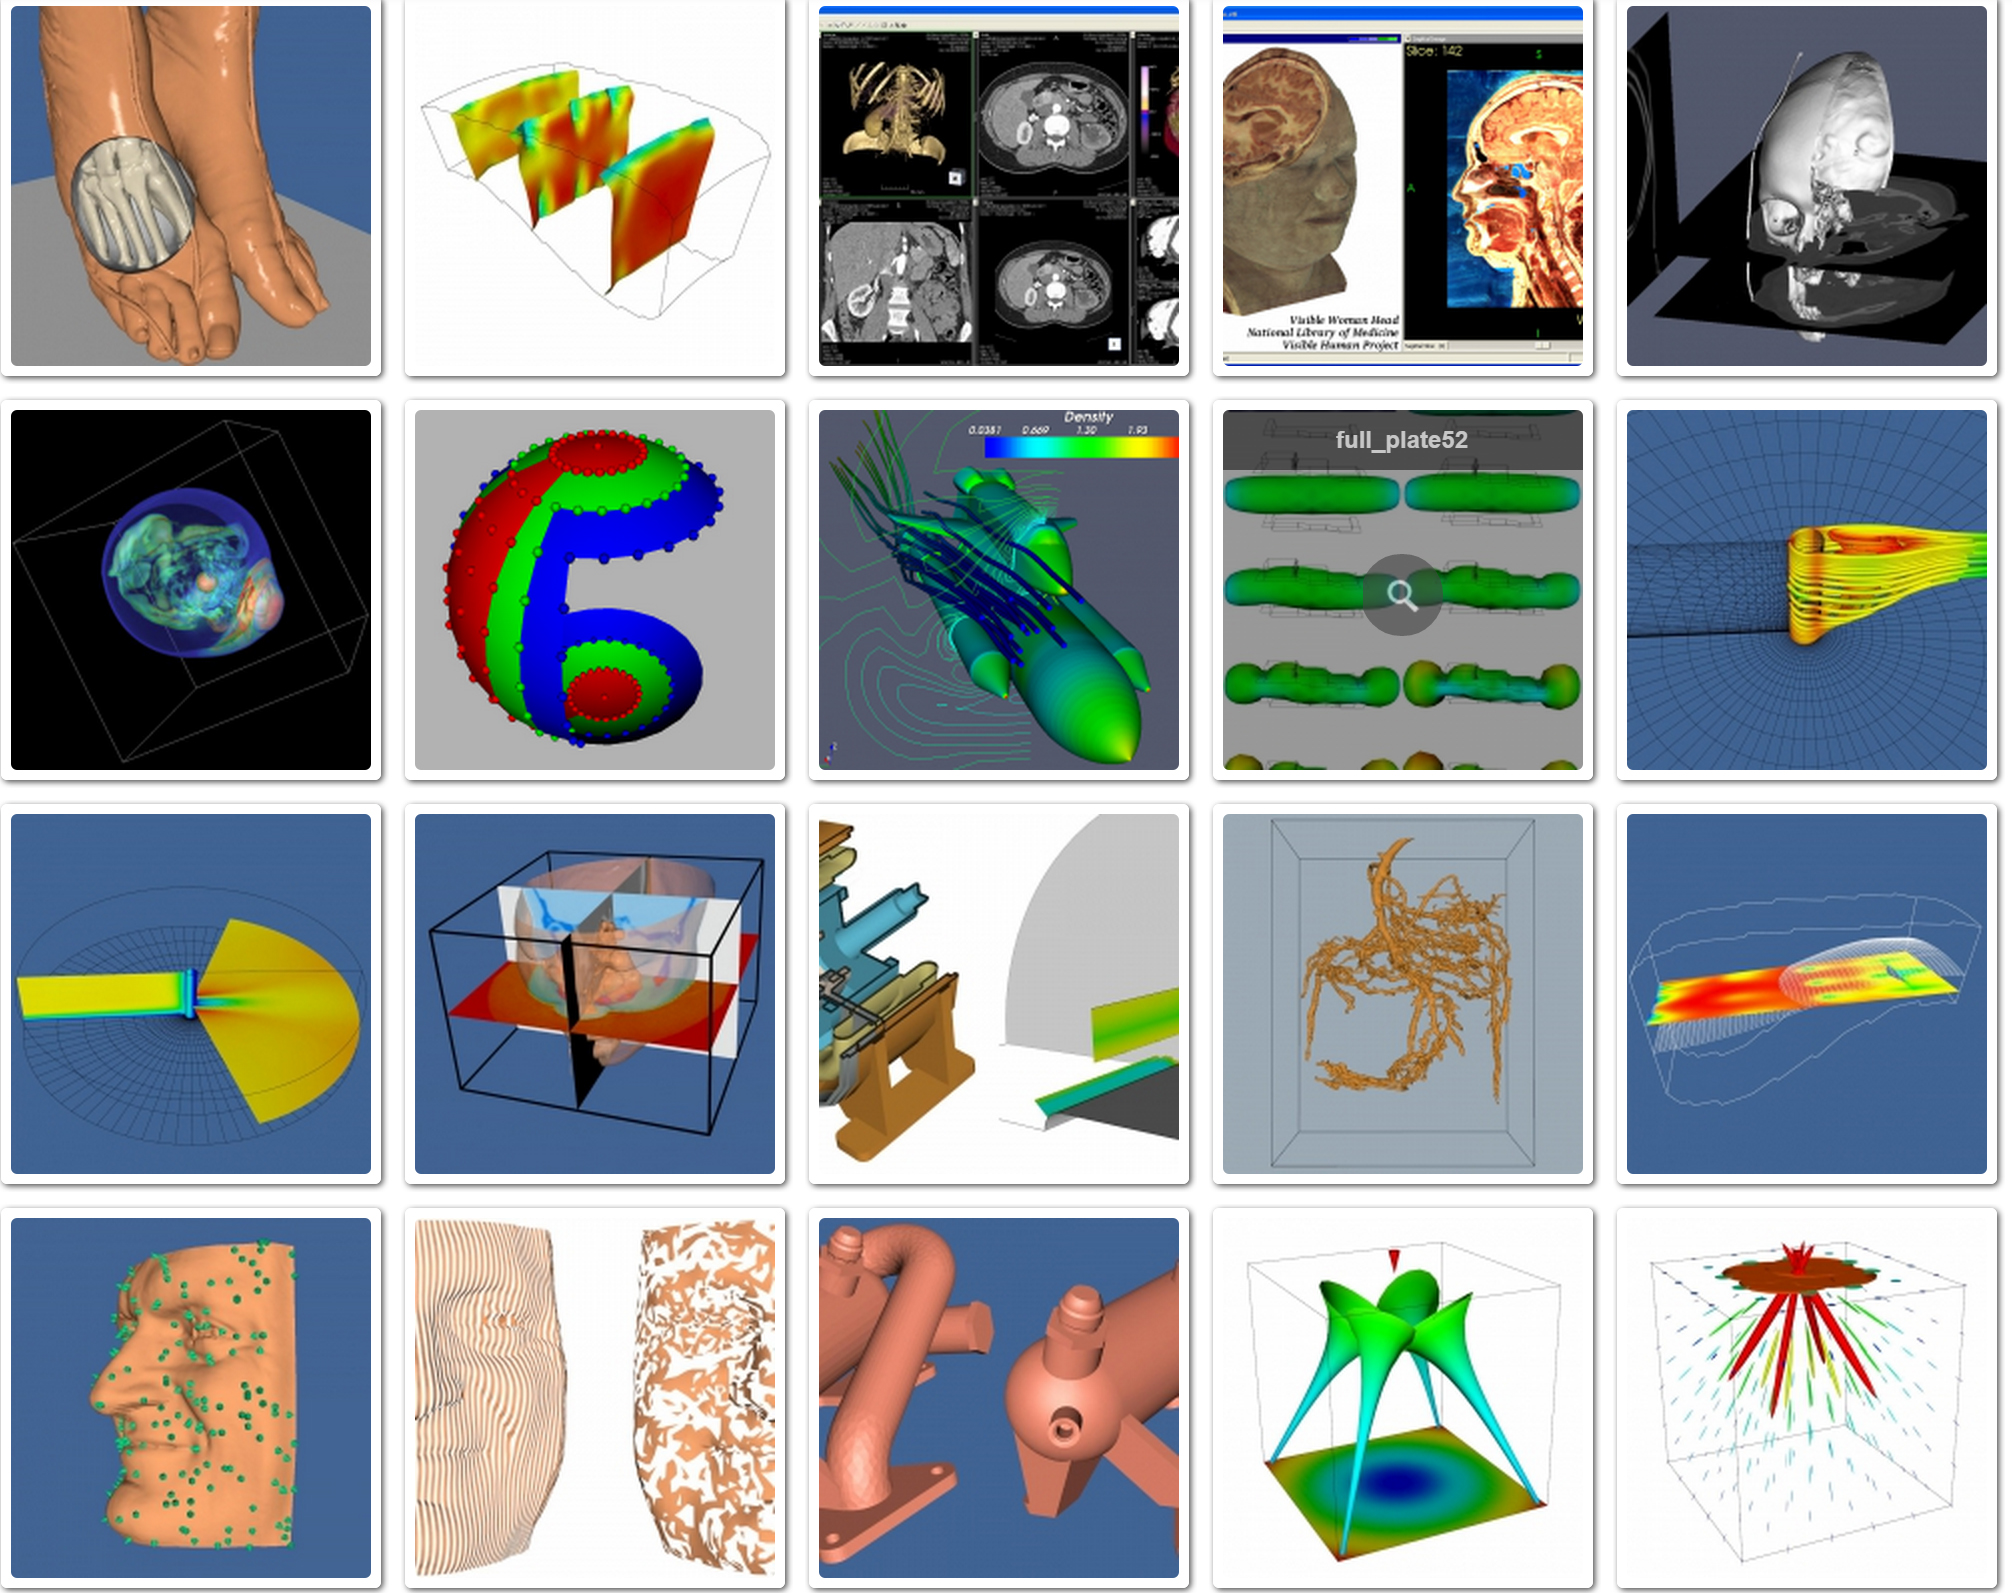
\includegraphics[width=0.9\linewidth]{graphics/vtk.jpg}
    \captionof{figure}[VTK Capabilities]{Different visualizations done with VTK.}
    \label{fig:vtkgallery}
\end{minipage}
VTK is probably the most advanced scientific visualization library, with a huge amount of visualization types. In figure \ref{fig:vtkgallery} you can see some of the visualization forms taken from the VTK gallery\cite{VTKGallery}.

It shares many of its goals with Romeo, namely \cite{Paraview}
\begin{itemize}
	\item Develop an open-source, multi-platform visualization application.
	\item Support distributed computation models to process large data sets.
	\item Create an open, flexible, and intuitive user interface.
	\item Develop an extensible architecture based on open standards.
\end{itemize}
VTK is a very big project and in this sense not really comparable to Romeo.
It amounts to a total of 3.642.105 lines of code written in 29 languages. The statistics can be found in table \ref{table:ParaviewStatistic} and \ref{table:VTKStatistic}.
The biggest difference is, that Romeo is implemented in a scientific programming language, while VTK is mainly implemented in C++.
This has two big implications:
Firstly, if the language doesn't have native C++ compatible data types and an overhead less C++ interface, shipping a large stream of data to VTK becomes slow.
Secondly, one must know C++ to extend VTK. This makes it difficult to create customized visualizations.